\documentclass[tikz,border=5mm]{standalone}
\usepackage{xcolor}

\definecolor{gameblue}{RGB}{0, 102, 204}
\definecolor{gamered}{RGB}{204, 51, 34}

\begin{document}
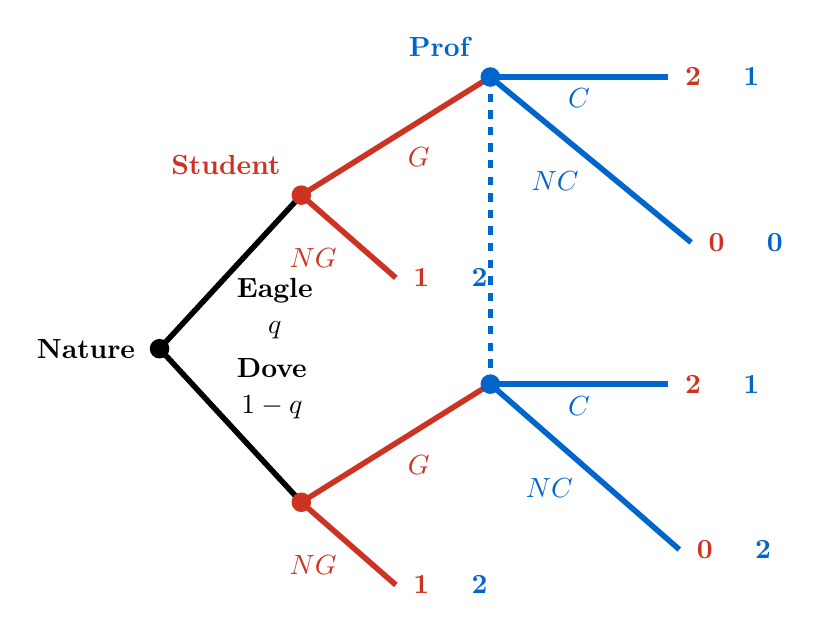
\begin{tikzpicture}[
    scale=1.5,
    font=\bfseries,
    dot/.style={circle, fill=#1, inner sep=2.5pt},
    dot/.default=black,
    line width=2pt
]

    % --- Coordinates ---
    % Nature Root
    \coordinate (nature)   at (0, 0);

    % Top Subtree (Eagle)
    \coordinate (t_you)     at (1.2, 1.3);
    \coordinate (t_qg)      at (2.8, 2.3);
    \coordinate (t_ng)      at (2.0, 0.6);
    \coordinate (t_leaf_c)  at (4.3, 2.3);
    \coordinate (t_leaf_nc) at (4.5, 0.9);

    % Bottom Subtree (Dove)
    \coordinate (b_you)     at (1.2, -1.3);
    \coordinate (b_qg)      at (2.8, -0.3);
    \coordinate (b_ng)      at (2.0, -2.0);
    \coordinate (b_leaf_c)  at (4.3, -0.3);
    \coordinate (b_leaf_nc) at (4.4, -1.7);

    % --- Level 0: Nature Branches ---
    \draw[black] (nature) -- (t_you) node[midway, below right, align=center, xshift=-2pt, yshift=2pt] {Eagle\\[1pt]$q$};
    \draw[black] (nature) -- (b_you) node[midway, above right, align=center, xshift=-2pt, yshift=-2pt] {Dove\\[1pt]$1-q$};

    % --- Level 1: "You" Branches (Red) ---
    \draw[gamered] (t_you) -- (t_qg) node[midway, below right] {$G$};
    \draw[gamered] (t_you) -- (t_ng) node[midway, below left] {$NG$};

    \draw[gamered] (b_you) -- (b_qg) node[midway, below right] {$G$};
    \draw[gamered] (b_you) -- (b_ng) node[midway, below left] {$NG$};

    % --- Information Set (Dashed Line connecting QG nodes) ---
    \draw[gameblue, dashed, line width=2pt] (t_qg) -- (b_qg);

    % --- Level 2: "QG" Branches (Blue) ---
    \draw[gameblue] (t_qg) -- (t_leaf_c)  node[midway, below] {$C$};
    \draw[gameblue] (t_qg) -- (t_leaf_nc) node[midway, below left] {$NC$};

    \draw[gameblue] (b_qg) -- (b_leaf_c)  node[midway, below] {$C$};
    \draw[gameblue] (b_qg) -- (b_leaf_nc) node[midway, below left] {$NC$};

    % --- Nodes & Decision Labels ---
    \node[dot=black, label={[black]left:Nature}] at (nature) {};

    \node[dot=gamered, label={[gamered]above left:Student}] at (t_you) {};
    \node[dot=gamered] at (b_you) {};

    \node[dot=gameblue, label={[gameblue]above left:Prof}] at (t_qg) {};
    \node[dot=gameblue] at (b_qg) {};

    % --- Payoffs: Red (You) \quad Blue (QG) ---
    % Top tree payoffs
    \node[right=2pt] at (t_ng)      {\textcolor{gamered}{1} \quad \textcolor{gameblue}{2}};
    \node[right=2pt] at (t_leaf_c)  {\textcolor{gamered}{2} \quad \textcolor{gameblue}{1}};
    \node[right=2pt] at (t_leaf_nc) {\textcolor{gamered}{0} \quad \textcolor{gameblue}{0}};

    % Bottom tree payoffs
    \node[right=2pt] at (b_ng)      {\textcolor{gamered}{1} \quad \textcolor{gameblue}{2}};
    \node[right=2pt] at (b_leaf_c)  {\textcolor{gamered}{2} \quad \textcolor{gameblue}{1}};
    \node[right=2pt] at (b_leaf_nc) {\textcolor{gamered}{0} \quad \textcolor{gameblue}{2}};

\end{tikzpicture}
\end{document}
